\section{Conclusion}
\label{sec:Conclusion}


\begin{figure}[t]
\centering
%%
\begin{subfigure}[t]{0.72\linewidth}
\centering
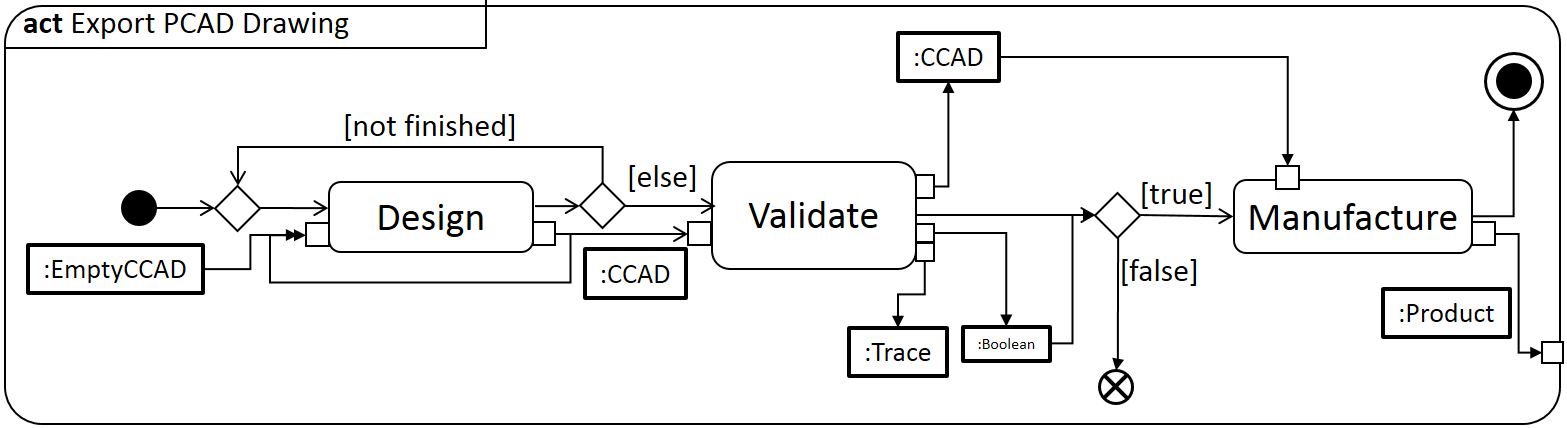
\includegraphics[width=0.98\textwidth]{CCAD_PM}
%\caption{$\mathsf{PM_{Full}}$: a possible \textsc{Pm} manufacturing 
%\textsc{CCad} designs at the expanse of your company!}
\phantomcaption{} 
\label{fig:CCAD-PM-Full}%
\end{subfigure}
%%
\begin{subfigure}[t]{0.23\linewidth}
\centering
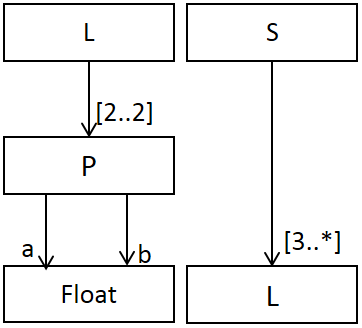
\includegraphics[width=\textwidth]{CCAD_Props}
%\caption{$\mbox{CAD}_1$ and $\mbox{CAD}_2$ pattern properties.}
\phantomcaption{}
\label{fig:PatternProperties}
\end{subfigure}
%%
\vspace{-1em}
\caption{(Left) Candidate \textsc{Pm} for manufacturing \textsc{CCad} designs.
(Right) Pattern properties for $\mbox{CAD}_1$ and $\mbox{CAD}_2$.}

\vspace{-0.5cm}
\end{figure}

To deal with the complexities in designing \textsc{cps}, \textsc{mpm} 
is seen as a potential candidate for helping project managers and engineers. 

This paper motivated the need of \textsc{mpm} for \textsc{cps} and identified 
three important dimensions: formalisms / languages; 
abstractions / viewpoints; and processes. It proposes, as a first step, a 
partial formalisation of two of these to capture the notion of paradigm: after 
defining the core characterising properties of a paradigm, we offer a decision procedure 
to check that a structure comprising two of the three previous dimensions 
satisfy these properties. This was illustrated with a (simplified) \textsc{cad} 
paradigm. 
%%
Many directions still need to be explored: adding multi-view properties as well as going from a single to multiple 
paradigms as well as specifying how they relate to each other (through 
abstractions/multiviews) and characterising such relationships; then validating 
the approach on realistic/industrial \textsc{cps} examples. 

% First, integrating the last 
% dimension is crucial to provide a general, multi-view and multi-concern picture 
% of a paradigm. Then, characterising how several paradigms may be combined is 
% another corner step towards formalising \textsc{mpm}. Finally, exploring more 
% theoretical questions like the difference between multi-formalisms and 
% multi-paradigms, the fact that \textsc{mpm} may be seen as a multi-paradigm 
% approach itself, remains important steps to consolidate our work. Finally, 
% applying our general framework on more realistic settings in \textsc{cps} is 
% required to validate our approach.

% presented a first step towards the full formalisation of 
% \textsc{mpm}, namely the languages/formalisms, the abstractions/relationships
% 
% We have presented a formalization of the notion of modeling paradigm 
% and illustrated it with the simple CAD paradigm. It consists of a set of 
% properties that can be evaluated on a modeling scenario to check if its 
% formalisms and workflows exhibit the features characterizing the paradigm. Like 
% for programming languages, formalizing modeling paradigms can help understanding 
% modeling approaches and guide implementation of modeling scenarios of different 
% contexts based on well- known paradigms.
% 
% Future work will consist of applying our definition to more complex modeling scenarios such as the ones for developing CPSs and further validate our definition and evaluate its usefulness. Furthermore, the composition of modeling paradigms can be studied to answers questions such as how to combine paradigms, and if such combinations are paradigms themselves.
% 

